\documentclass{standalone}
    \usepackage{tikz}
    \begin{document}

    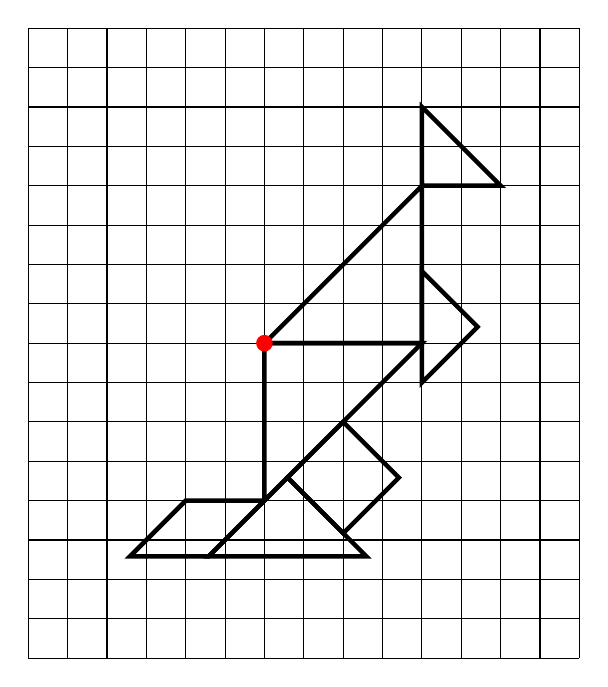
\begin{tikzpicture}
    \draw[step=5mm] (-3,-4) grid (4,4);
    \draw[ultra thick] ({2},{2}) -- ({2},{3}) -- ({3},{2}) -- cycle;
\draw[ultra thick] ({2},{-1/2+1*sqrt(2)}) -- ({2+1/2*sqrt(2)},{-1/2+1/2*sqrt(2)}) -- ({2},{-1/2}) -- cycle;
\draw[ultra thick] ({0},{0}) -- ({2},{2}) -- ({2},{0}) -- cycle;
\draw[ultra thick] ({1-1/2*sqrt(2)},{-1-1/2*sqrt(2)}) -- ({1},{-1}) -- ({1+1/2*sqrt(2)},{-1-1/2*sqrt(2)}) -- ({1},{-1-1*sqrt(2)}) -- cycle;
\draw[ultra thick] ({0},{-2}) -- ({0},{0}) -- ({2},{0}) -- cycle;
\draw[ultra thick] ({-1/2*sqrt(2)},{-2-1/2*sqrt(2)}) -- ({1-1/2*sqrt(2)},{-1-1/2*sqrt(2)}) -- ({2-1/2*sqrt(2)},{-2-1/2*sqrt(2)}) -- cycle;
\draw[ultra thick] ({-1-1/2*sqrt(2)},{-2-1/2*sqrt(2)}) -- ({-1},{-2}) -- ({0},{-2}) -- ({-1/2*sqrt(2)},{-2-1/2*sqrt(2)}) -- cycle;
    \fill[red] (0,0) circle (3pt);
    \end{tikzpicture}

    \end{document}